% Este archivo es parte de la presentación de libWiiEsp, protegida bajo la 
% licencia GFDL. Copyright (C) 2011 Ezequiel Vázquez de la Calle

% -*-desarrollo.tex-*-

\section{Desarrollo del proyecto}

\subsection{Cómo programar para Nintendo Wii}

\begin{frame}	
\frametitle{Programar para Nintendo Wii}
	\begin{block}{\textit{Big Endian}}
		\begin{figure}[H]
			\label{endianess}
			\begin{center}
			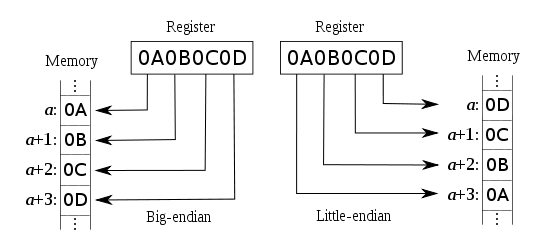
\includegraphics[scale=0.50]{endianess.png}
			\end{center}
			\caption{Diferencias entre \textit{Big Endian} y \textit{Little Endian}}
		\end{figure}
	\end{block}
\end{frame}

\begin{frame}	
\frametitle{Programar para Nintendo Wii}
	\begin{block}{Alineación de los datos}
		\begin{figure}[H]
			\label{alineacion}
			\begin{center}
			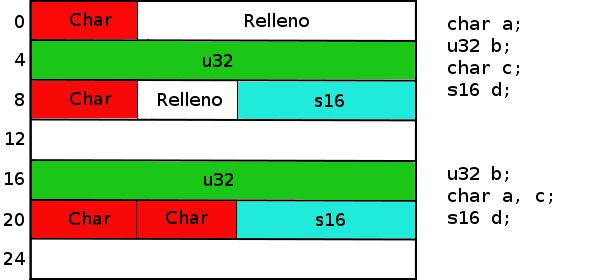
\includegraphics[scale=0.50]{alineacion.png}
			\end{center}
			\caption{Estado de la memoria, alineando o no los datos}
		\end{figure}
	\end{block}
\end{frame}

\begin{frame}	
\frametitle{Programar para Nintendo Wii}
	\begin{block}{Otras consideraciones}
		\begin{itemize}
		\item Alineación y relleno al leer desde un periférico: 32 bytes.
		\item Cantidad de memoria: Wii tiene 64 MB de RAM.
		\item Lanzar un programa: Homebrew Channel.
		\item Tipos de datos.
		\end{itemize}
		\begin{figure}[H]
			\label{tiposdatos}
			\begin{center}
			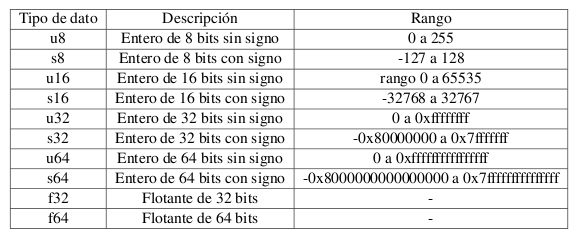
\includegraphics[scale=0.4]{tiposdatos.png}
			\end{center}
			\caption{Tipos de datos utilizados en Nintendo Wii}
		\end{figure}
	\end{block}
\end{frame}

\subsection{Necesidades detectadas}

\begin{frame}	
\frametitle{Necesidades detectadas}
	\begin{block}{Controlar sistemas de la videoconsola}
		\begin{itemize}
			\item Sistema gráfico.
			\begin{itemize}
				\item Dibujo de texturas.
				\item Escritura con fuentes de texto.
			\end{itemize}
			\item Sistema de audio: música y efectos de sonido.
			\item Controladores \textit{Wii Remote}.
			\item Medios de almacenamiento: tarjeta SD.
		\end{itemize}
	\end{block}
	\begin{figure}[H]
		\label{texturas}
		\begin{center}
		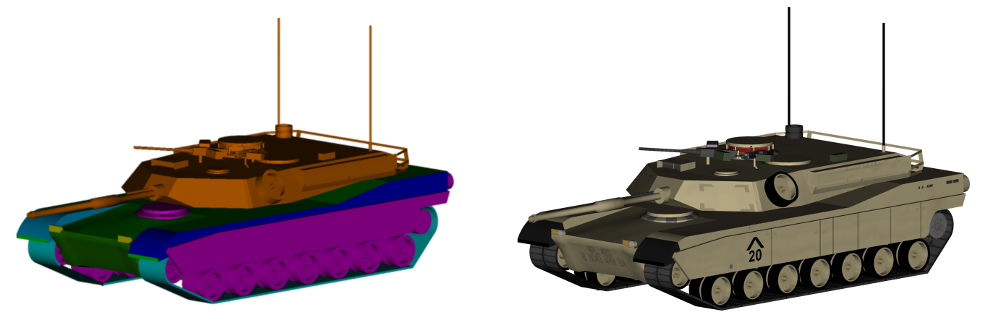
\includegraphics[scale=0.25]{texturas.png}
		\end{center}
		\caption{Figura 3D sin texturas y con texturas}
	\end{figure}
\end{frame}

\begin{frame}	
\frametitle{Necesidades detectadas}
	\begin{block}{Otros módulos con funcionalidad necesaria}
		\begin{itemize}
			\item Analizador XML.
			\item Organizar los recursos multimedia.
			\item Reproducción de animaciones.
			\item Soporte de internacionalización.
			\item Detección de colisiones.
			\item Registro de mensajes del sistema.
		\end{itemize}
	\end{block}
\end{frame}

\begin{frame}	
\frametitle{Necesidades detectadas}
	\begin{block}{Elementos de un juego 2D}
		\begin{itemize}
			\item Actor: elemento con entidad propia dentro del juego.
			\item Escenario: mundo en el que los actores interactúan.
		\end{itemize}
	\end{block}
	\begin{block}{Plantillas}
		\begin{itemize}
			\item Abstraen de los detalles comunes de estos elementos.
			\item Plantilla para actores: base para definir comportamiento.
			\item Plantilla para escenarios: crear niveles de forma sencilla.
			\item Plantilla para clase principal: inicialización de la videoconsola.
		\end{itemize}
	\end{block}
\end{frame}

\begin{frame}	
\frametitle{Necesidades detectadas}
	\begin{block}{Documentación amplia y útil}
		\noindent Facilitar el aprendizaje por medio de documentación.
		\begin{itemize}
			\item Manual de instalación y uso. (34 páginas)
			\item Manual de referencia completo. (Generado con Doxygen)
			\item Memoria del proyecto. (243 páginas)
		\end{itemize}
	\end{block}
	\pause
	\begin{block}{Ejemplos didácticos}
		\noindent Ilustrar el funcionamiento de la biblioteca.
		\begin{itemize}
			\item \textbf{Arkanoid Wii}: romper ladrillos con una bola.
			\item \textbf{Duck Hunt Wii}: cazar patos que aparecen en la pantalla.
			\item \textbf{Wii Pang}: personaje rompe pompas con ganchos verticales.
		\end{itemize}
	\end{block}
\end{frame}

\subsection{Metodología}

\begin{frame}
\frametitle{Metodología}
	\begin{itemize}
		\item Metodología iterativa, basada en \textit{Rational Unified Proccess}.
		\item Por cada etapa se construye un módulo completo.
	\end{itemize}
	\pause
	\begin{block}{Características del sistema}
		\begin{itemize}
			\item Totalmente orientado a objetos.
			\item Separación completa de código fuente y datos: XML.
			\item Fase de diseño:
			\begin{itemize}
				\item Patrón \textit{Singleton}: para los módulos con una única instancia.
				\item Patrón Visitante: para la implementación de \textit{Double Dispatch} en el módulo de colisiones.
			\end{itemize}
		\end{itemize}
	\end{block}
\end{frame}

\subsection{Detalles de implementación}

\begin{frame}
\frametitle{Detalles de implementación}
	\begin{block}{Proyección ortográfica}
		\begin{itemize}
			\item Foco de luz en el infinito.
			\item Proyectar perpendicularmente a la pantalla.
			\item No hay cambios de tamaño por distancia al plano.
		\end{itemize}
	\end{block}
	\begin{figure}[H]
		\label{ortho}
		\begin{center}
		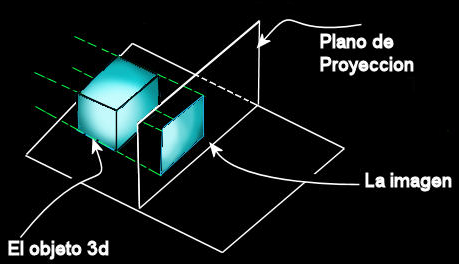
\includegraphics[scale=0.4]{ortho.png}
		\end{center}
		\caption{Proyección ortográfica}
	\end{figure}
\end{frame}

\begin{frame}
\frametitle{Detalles de implementación}
	\begin{block}{Doble búfer}
		\begin{itemize}
			\item Dos zonas de memoria para dibujar fotogramas.
			\item Se consigue evitar parpadeos al mostrar animaciones.
		\end{itemize}
	\end{block}
	\begin{figure}[H]
		\label{doblebuffer}
		\begin{center}
		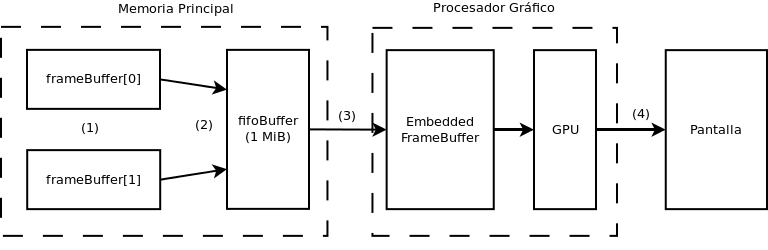
\includegraphics[scale=0.4]{doblebuffer.png}
		\end{center}
		\caption{Esquema del sistema gráfico con doble búfer}
	\end{figure}
\end{frame}

\begin{frame}
\frametitle{Detalles de implementación}
	\begin{block}{Formato de vídeo RGB5A3}
		\begin{itemize}
		\item Formato nativo con el que trabaja el procesador gráfico.
		\item Permite trabajar cómodamente con transparencias.
		\end{itemize}
	\end{block}
	\begin{figure}[H]
		\label{rgb5a3}
		\begin{center}
		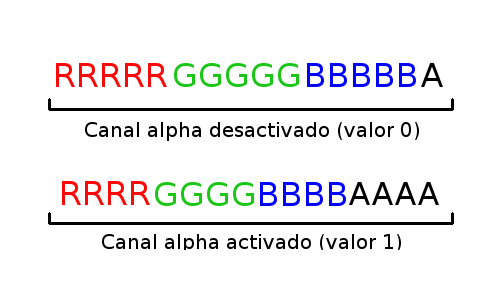
\includegraphics[scale=0.45]{rgb5a3.png}
		\end{center}
		\caption{Formato de píxel RGB5A3}
	\end{figure}
\end{frame}

\begin{frame}
\frametitle{Detalles de implementación}
	\begin{block}{Texturas organizadas en \textit{tiles}}
		\begin{itemize}
			\item Píxeles adyacentes en la imagen, también en memoria.
			\item GPU usa texturas en tiles para trabajar de forma optimizada.
		\end{itemize}
	\end{block}
	\begin{figure}[H]
		\label{texturatiles}
		\begin{center}
		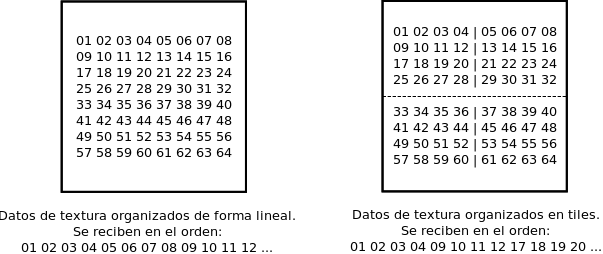
\includegraphics[scale=0.45]{texturatiles.png}
		\end{center}
		\caption{Textura lineal y textura organizada en \textit{tiles} de 4x4}
	\end{figure}
\end{frame}

\begin{frame}
\frametitle{Detalles de implementación}
	\begin{block}{Sistema de audio}
		\begin{itemize}
		\item Procesador DSP dedicado únicamente al control de audio.
		\item Reproduce hasta 16 flujos de sonido (voces) simultáneamente.
		\item Una voz reservada para pistas de música.
		\item Formato nativo de Wii:
			\begin{itemize}
			\item 48000 Hz.
			\item Estéreo (dos canales).
			\item \textit{Samples} de 16 bits con signo.
			\end{itemize}
		\end{itemize}
	\end{block}
\end{frame}

\begin{frame}
\frametitle{Detalles de implementación}
	\begin{block}{Fuentes de texto}
		\begin{itemize}
		\item \textit{FreeType2} genera una imagen \textit{bitmap} para cada carácter.
		\item Mapa de bits monocromo: un píxel se dibuja si tiene valor 1.
		\item En pantalla se dibuja cada carácter píxel a píxel.
		\end{itemize}
	\end{block}
	\begin{figure}[H]
		\label{fuentestexto}
		\begin{center}
		
\includegraphics[scale=0.45]{fuentestexto.png}
		\end{center}
		\caption{Mapa de bits monocromo asociado al caracter \textit{a}}
	\end{figure}
\end{frame}

\begin{frame}
\frametitle{Detalles de implementación}
	\begin{block}{Colisiones: Técnica de \textit{Double Dispatch}}
		\noindent Evita tener que identificar el tipo de dos objetos derivados de la misma clase base.
	\end{block}
	\begin{figure}[H]
		\label{doubledispatch}
		\begin{center}
		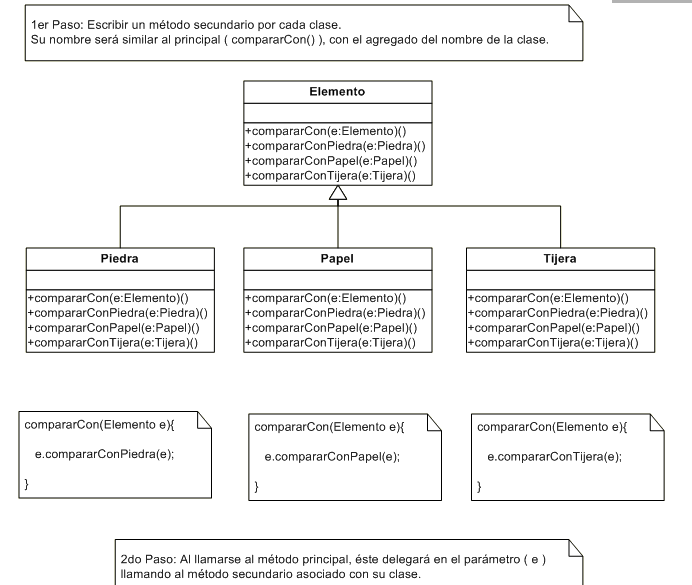
\includegraphics[scale=0.40]{doubledispatch.png}
		\end{center}
	\end{figure}
\end{frame}

\begin{frame}
\frametitle{Detalles de implementación}
	\begin{block}{Escenarios: Mapas de \textit{tiles}}
		\noindent \textbf{Tile}: una imagen cuadrada, rectangular o hexagonal, utilizada para generar imágenes de mayor complejidad.
	\end{block}
	\begin{figure}[H]
		\label{tileset}
		\begin{center}
		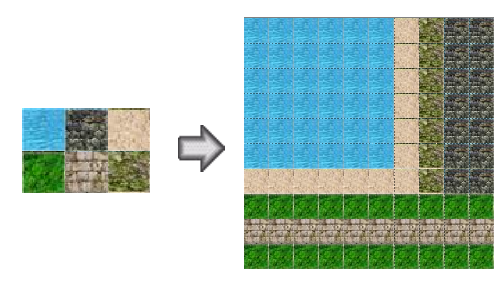
\includegraphics[scale=0.4]{tileset.png}
		\end{center}
		\caption{\textit{Tileset} (conjunto de \textit{tiles}) y mapa de \textit{tiles}}
	\end{figure}
\end{frame}

\subsection{Herramientas utilizadas}

\begin{frame}
\frametitle{Herramientas utilizadas}
	\begin{block}{Tecnología}
		\begin{itemize}
			\item C++, con GNU Make.
			\item XML
		\end{itemize}
	\end{block}
	\begin{block}{Desarrollo}
		\begin{itemize}
			\item \textbf{Gimp}: edición de imágenes.
			\item \textbf{SoX}: edición de sonido.
			\item \textbf{Doxygen}: documentación automática de código.
			\item \textbf{\LaTeX}: sistema de composición de textos.
			\item \textbf{Gantt Project}: diagramas de planificación.
			\item \textbf{Dia}: editor de diagramas UML.
			\item \textbf{Cppcheck}: analizador estático de código fuente C++.
			\item \textbf{Subversion}: control de revisiones.
			\item \textbf{Tiled}: editor de mapas de \textit{tiles}.
		\end{itemize}
	\end{block}
\end{frame}

\begin{frame}
\frametitle{Herramientas utilizadas}
	\begin{block}{DevKitPPC}
		\begin{itemize}
			\item Generación de ejecutables para sistemas \textit{Power PC}.
			\item Reglas de compilación específicas para Wii.
			\item Fácilmente ampliable con bibliotecas externas.
			\item \textbf{Wiiload}: lanzar ejecutables mediante red local.
		\end{itemize}
	\end{block}
	\begin{block}{Bibliotecas externas}
		\noindent Previamente adaptadas para trabajar con \textit{DevKitPPC}.
		\begin{itemize}
			\item \textbf{Libogc}: permite acceder al hardware de Nintendo Wii.
			\item \textbf{Libfat}: para trabajar con particiones FAT/FAT32
			\item \textbf{FreeType2}: necesaria para utilizar fuentes de texto.
			\item \textbf{TinyXml}: proporciona una interfaz para trabajar con XML.
		\end{itemize}
	\end{block}
\end{frame}

\subsection{Pruebas y validación}

\begin{frame}
\frametitle{Pruebas y validación}
	\begin{block}{Especificación de las pruebas}
		\begin{itemize}
			\item Garantizar el buen funcionamiento de la herramienta.
			\item Se han realizado durante y después del desarrollo.
			\item Han consistido en varios grupos de pruebas:
			\begin{itemize}
				\item Pruebas de módulo.
				\item Pruebas de sistema.
				\item Pruebas de \textit{makefile}.
				\item Pruebas de juegos.
				\item Análisis estático del código con \textit{Cppcheck}.
			\end{itemize}
			\item Todas las pruebas se han realizado sobre la videoconsola.
		\end{itemize}
	\end{block}
\end{frame}

\begin{frame}
\frametitle{Pruebas y validación}
	\begin{block}{Pruebas de módulo}
		\noindent Prueba exhaustiva de cada módulo, tras finalizar su desarrollo:
		\begin{itemize}
			\item Caja blanca: comprobar los distintos caminos que toma el flujo de ejecución en el módulo.
			\item Caja negra: partiendo de conjuntos de datos de entrada y comprobando la salida que producen.
		\end{itemize}
	\end{block}
	\pause
	\begin{block}{Pruebas de sistema}
		\noindent Comprobar funcionamiento de cada módulo junto con los demás.
		\begin{itemize}
			\item Animación e Imagen.
			\item Galería y recursos multimedia.
			\item Actor y figuras de colisión.
			\item Etc.
		\end{itemize}
	\end{block}
\end{frame}

\begin{frame}[fragile]
\frametitle{Pruebas y validación}
	\begin{block}{Pruebas de \textit{makefile}}
		\begin{itemize}
			\item Compilación.
			\item Generación de documentación.
			\item Empaquetado.
			\item Instalación y desinstalación.
		\end{itemize}
	\end{block}
	\begin{block}{Pruebas de juegos}
		\begin{itemize}
			\item \textit{Playtesting}: varias personas juegan y reportan errores.
		\end{itemize}
	\end{block}
	\begin{block}{Análisis estático de código fuente}
		\begin{itemize}
			\item Se utilizó Cppcheck.
			\item \begin{lstlisting}{style=C, frame=none}
				> cppcheck --enable=all include src
			\end{lstlisting}
		\end{itemize}
	\end{block}
\end{frame}

\begin{frame}
\frametitle{Pruebas y validación}
	\begin{block}{Problemas surgidos durante el desarrollo}
		\begin{itemize}
			\item Poca documentación existente: tutoriales muy incompletos.
			\item Control de la eficiencia: hardware limitado.
			\item Trabajo a bajo nivel con recursos: imágenes y fuentes.
			\item Difícil depuración.
		\end{itemize}
	\end{block}
	\begin{figure}[H]
		\label{excepcion}
		\begin{center}
		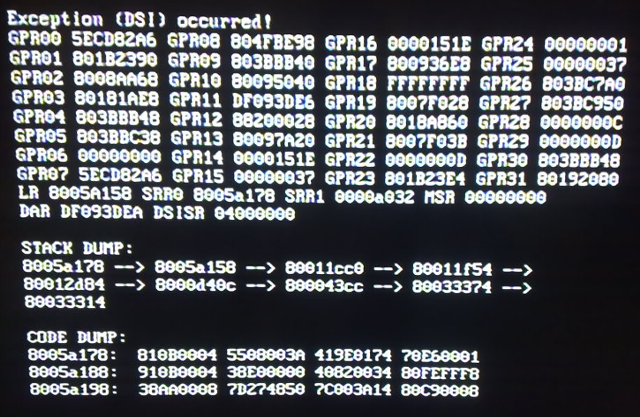
\includegraphics[scale=0.3]{excepcion.png}
		\end{center}
	\end{figure}
\end{frame}

